\begin{frame}
\begin{tabular}{cc}
\psset{xunit=0.35cm,yunit=0.35cm}
\begin{pspicture*}(-7,-10)(7,10)
\psaxes[labels=none, ticks=x, Dx=1.570796327] {<->}(0,0)(-5.5,-10)(5.5,10)
\tiny
\rput[lt](5.5,0){$x$}
\rput[lb](0.2,9){$y$}
%\rput[t](1,-0.1){1}
\psline[linecolor=gray](1,-0.1)(1,0.1) % x unit mark
\rput[lb](1.570796327,0.1){$\frac{\pi}2$}
\psline[linecolor=gray](1.570796327,-0.1)(1.570796327,0.1) % pi/2 unit mark
%\rput[br](0,1){1}
\psline[linecolor=gray](-0.1,1)(0.1,1) % y unit mark

\psplot[linecolor=red]{-1.57}{1.57}{ 180 x mul  3.1415 div tan} 
\psplot[linecolor=red]{-4.71}{-1.58}{ 180 x mul  3.1415 div tan} 
\psplot[linecolor=red]{1.58}{4.71}{ 180 x mul  3.1415 div tan} 

\psline[linestyle=dotted](-4.71238898,-10)(-4.71238898,10)
\psline[linestyle=dotted](-1.570796327,-10)(-1.570796327,10)
\psline[linestyle=dotted](1.570796327,-10)(1.570796327,10)
\psline[linestyle=dotted](4.71238898,-10)(4.71238898,10)
\end{pspicture*}
%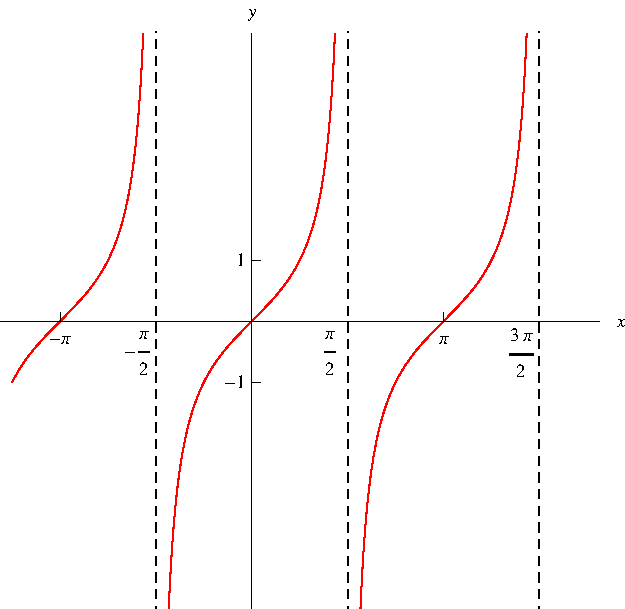
\includegraphics[width=5.5cm]{trigonometry/pictures/app-d-tan.pdf}%

&%
\psset{xunit=0.35cm,yunit=0.35cm}
\begin{pspicture*}(-7,-10)(8,10)
\psaxes[labels=none, ticks=x, Dx=1.570796327] {<->}(0,0)(-7,-10)(7,10)
\tiny
\rput[lt](7,0){$x$}
\rput[lb](0.2,9){$y$}
%\rput[t](1,-0.1){1}
\psline[linecolor=gray](1,-0.1)(1,0.1) % x unit mark
\rput[rb](3.13,0.1){$\pi$}
\psline[linecolor=gray](1.570796327,-0.1)(1.570796327,0.1) % pi/2 unit mark
%\rput[br](0,1){1}
\psline[linecolor=gray](-0.1,1)(0.1,1) % y unit mark

\psplot[linecolor=red]{0.01}{3.14}{1 180 x mul  3.1415 div tan div} 
\psplot[linecolor=red]{3.15}{6.28}{1 180 x mul  3.1415 div tan div} 
\psplot[linecolor=red]{-3.14}{-0.01}{1 180 x mul  3.1415 div tan div} 
\psplot[linecolor=red]{-6.28}{-3.15}{1 180 x mul  3.1415 div tan div} 
%\psplot[linecolor=red]{-4.71}{-1.58}{ 180 x mul  3.1415 div cot} 
%\psplot[linecolor=red]{1.58}{4.71}{ 180 x mul  3.1415 div cot} 

\psline[linestyle=dotted](-6.283185307,-10)(-6.283185307,10)
\psline[linestyle=dotted](-3.141592654,-10)(-3.141592654,10)
\psline[linestyle=dotted](3.141592654,-10)(3.141592654,10)
\psline[linestyle=dotted](6.283185307,-10)(6.283185307,10)
\end{pspicture*}
%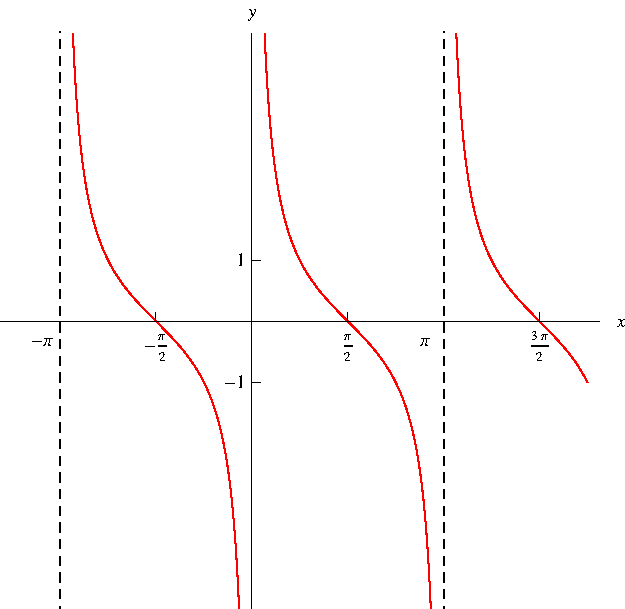
\includegraphics[width=5.5cm]{trigonometry/pictures/app-d-cot.pdf}%
\\%
$y = \tan x$ & $y = \cot x$\\
\end{tabular}
\end{frame}
